% Slides for the final presentation of the thesis on the December 3, 2014.

\documentclass{beamer}
\usetheme{default}
\setbeamertemplate{navigation symbols}{}
\setbeamertemplate{footline}[frame number]

\usepackage{listings}
\usepackage{textcomp}
\usepackage{multicol}
\usepackage{tikz}
\usepackage{thmtools}

\usetikzlibrary{shapes,arrows,positioning}

\declaretheorem[thmbox=M]{definition}
\declaretheorem[thmbox=M]{example}

\newcommand{\textapprox}{\raisebox{0.5ex}{\texttildelow}}
\lstset{basicstyle=\ttfamily,literate={~}{\textapprox}{1}}

\newcommand{\code}{\lstinline[breaklines=true]}

\title{A Language for the Specification and Efficient Implementation
  of Type Systems}
\author{Pascal Wittmann}
\date{December 3, 2014}

% TODO: "apply" (of typing rules) is used in two different contexts
%         - pattern of the conclusion matches
%         - in addition premises are satisfied

\begin{document}

\begin{frame}[plain]
  \titlepage{}
\end{frame}

\begin{frame}
  \frametitle{Motivation}

  \begin{center}
    Goal: \textbf{Automatically} generate \textbf{efficient} type
    checkers from \textbf{high-level} specifications.
  \end{center}

  \begin{itemize}
  \item Type systems provide
    \begin{itemize}
    \item static approximation of program semantics
    \item means to establish and enforce abstraction barriers
    \item documentation in sync with source code
    \end{itemize}
  \item Domain Specific Languages (DSL) benefit from specialized type systems
  \item Gap between formal definitions of type systems and their
    implementations
  \end{itemize}
\end{frame}

\begin{frame}
  \frametitle{Research Problem}
  \begin{itemize}
  \item Type system specifications may be have rules that overlap in
    non-trivial ways
  \item Those overlaps require the type checker to backtrack
  \item Currently, type systems are transformed hand into algorithmic
    type systems
  \item Ensuring preservation of semantics requires non-trivial proofs
  \end{itemize}
  \begin{centering}
    How to remove overlap automatically while preserving the semantics?
  \end{centering}
\end{frame}

\begin{frame}[fragile]
  \frametitle{Optimization Strategies}
  \begin{example}
    Consider a subtyping relation on types \texttt{Int} and
    \texttt{Type -> Type}
    \begin{lstlisting}
               ~T1 <: ~S1
~S = ~T        ~S2 <: ~T2  
======== refl  ======================== arrow
~S <: ~T       ~S1 -> ~S2 <: ~T1 -> ~T2
    \end{lstlisting}
    Goal: Remove the overlap between rules \texttt{refl} and
    \texttt{arrow}.\\
  \end{example}
  General idea:
  \begin{itemize}
  \item Identify problematic rules
  \item Derive more specific versions of problematic rules
  \item Remove unnecessary rules
  \end{itemize}
\end{frame}

\begin{frame}[fragile]
  \frametitle{Strategy I: Unfolding}
  \begin{itemize}
  \item The problematic rule in this example is \texttt{refl}
    \begin{itemize}
    \item It is applicable to strictly more terms than \texttt{trans}
    \item It is applicable to all instances of the subtyping judgment
    \end{itemize}
  \item Idea: Unfold the structure of the variables in the conclusion
  \end{itemize}
\begin{lstlisting}
Int = Int           ~A -> ~B = Int 
========== R1       =============== R2
Int <: Int          ~A -> ~B <: Int
\end{lstlisting}
\begin{lstlisting}
Int = ~C -> ~D      ~A -> ~B = ~C -> ~D
=============== R3  ==================== R4
Int <: ~C -> ~D     ~A -> ~B <: ~C -> ~D
\end{lstlisting}
\end{frame}

\begin{frame}[fragile]
  \frametitle{Strategy II/III: Unsatisfiable \& Valid Premises}
  \begin{itemize}
  \item The unfolding of rules is purely syntactic
  \item Exploit semantics to unnecessary rules
    \begin{itemize}
    \item Remove valid premises from rules
      \begin{lstlisting}
Int = Int
========== R1
Int <: Int
      \end{lstlisting}
    \item Remove rules with unsatisfiable premises
      \begin{multicols}{2}
        \begin{lstlisting}
~A -> ~B = Int
=============== R2
~A -> ~B <: Int
        \end{lstlisting}
        \begin{lstlisting}
Int = ~C -> ~D
=============== R3
Int <: ~C -> ~D
        \end{lstlisting}
      \end{multicols}
    \end{itemize}
  \end{itemize}
\end{frame}

\begin{frame}[fragile]
  \frametitle{Strategy IV: Subsumption}
  \begin{definition}
    Rule $r_1$ \emph{subsumes} $r_2$ if they have the same conclusion (modulo
    variable renaming) and the premises of rule $r_2$ imply the
    conjunction of all premisses of $r_1$.
  \end{definition}
  
\begin{lstlisting}
                      ~C <: ~A
~A -> ~B = ~C -> ~D   ~B <: ~D
====================  ====================
~A -> ~B <: ~C -> ~D  ~A -> ~B <: ~C -> ~D
\end{lstlisting}

Is one of these rules subsumed by the other?

Conjecture: The left rule is subsumed by the right rule.
\end{frame}

\begin{frame}[fragile]
  \frametitle{Strategy IV: Subsumption}
  \begin{itemize}
  \item We can remove subsumed typing rules while preserving the
    semantics of the type system
    \begin{itemize}
    \item Both applicable to the same terms
    \item The subsuming rule is applicable whenever the subsumed rule is
    \end{itemize}
  \item Therefore we identify all subsumed rules and remove them
  \item Conjecture is proved by structural induction
    \begin{align*}
        \forall a, b, c, d \,.\, (a \text{ \code|->| } b = c \text{
          \code|->| } d) &\implies (
        c <: a \land b <: d)
    \end{align*}
  \item One case of the induction proof
\end{itemize}
% TODO Variable names & formatting
\small
\begin{align*}
  (a_1 \text{\code|->|} a_2) \text{\code|->|} \text{\code|Int|} = (c_1
  \text{\code|->|} c_2) \text{\code|->|} \text{\code|Int|} &\implies (
  c_1 \text{\code|->|} c_2 <: a_1 \text{\code|->|} a_2\land
  \text{\code|Int|} <: \text{\code|Int|}) \\
  ((a_1 \text{\code|->|} a_2) = (c_1 \text{\code|->|} c_2) \land
  \text{\code|Int|} = \text{\code|Int|}) &\implies (c_1
  \text{\code|->|} c_2 <: a_1 \text{\code|->|} a_2 \land
  \text{\code|Int|} <:
  \text{\code|Int|}) \\
  (a_1 \text{\code|->|} a_2) = (c_1 \text{\code|->|} c_2) &\implies
  c_1 \text{\code|->|} c_2 <: a_1 \text{\code|->|}
  a_2 \\
  (c_1 \text{\code|->|} c_2) = (a_1 \text{\code|->|} a_2) &\implies
  c_1 \text{\code|->|} c_2 <: a_1 \text{\code|->|}
  a_2 \\
  ((a_1 <: c_1) \land (c_2 <: a_2)) &\implies c_1 \text{\code|->|} c_2
  <: a_1 \text{\code|->|} a_2
\end{align*}
\end{frame}

\begin{frame}
  \frametitle{Implementation}
  \begin{itemize}
  \item From a type system specification we generate
    \begin{itemize}
    \item first-order formulas
    \item a type checker
    \end{itemize}
  \item We use automated theorem proving to prove the conjectures seen
    in the optimization strategies
  \item Generation of a type checker form optimized specifications
  \item First-order formulas serve in combination with automated
    theorem proving as a reference implementation
  \end{itemize}
  \begin{center}
  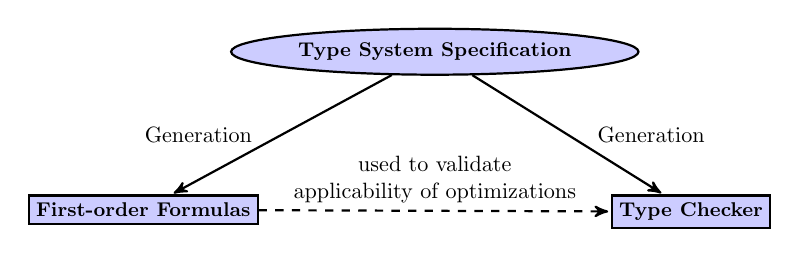
\begin{tikzpicture}[scale=.8,transform shape,->,>=stealth',shorten >=1pt,auto,align=center,node distance=1cm,thick,main node/.style={fill=blue!20,rectangle,draw,font=\small\bfseries}]
    \node[main node, style={ellipse}] (1) {Type System Specification};
    \node[main node] (2) [below left=2cm and .5cm of 1]  {First-order Formulas};
    \node[main node] (3) [below right=2cm and .5cm of 1] {Type Checker};

  \path[every node/.style={}]
  (1) edge node [outer sep=10pt,left] {Generation} (2)
  (1) edge node [outer sep=10pt,right] {Generation} (3);

  \path[every node/.style={}, dashed]
  (2) edge node [above] {used to validate \\ applicability of
    optimizations} (3);
  \end{tikzpicture}
  \end{center}
\end{frame}

\begin{frame}
  \frametitle{Type Checker}
  The type checker has four phases
  \begin{enumerate}
  \item Translation of typing rules into normalized templates
  \item Optimization of templates \checkmark{}
  \item Generation of constraints according to an expression
  \item Solving of the generated constraints
  \end{enumerate}
  \vspace{.5cm}
  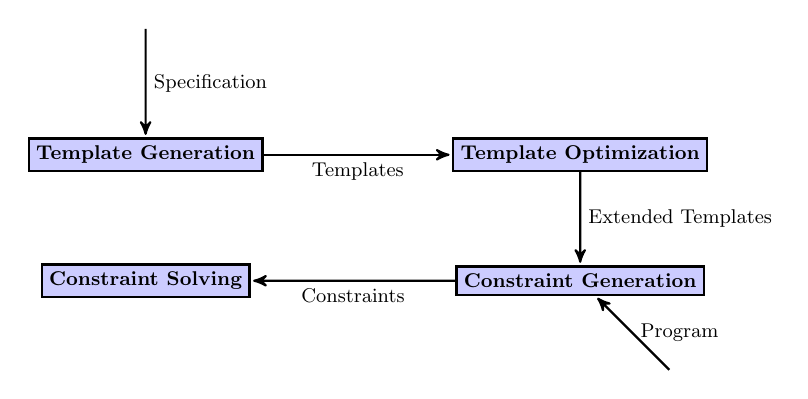
\begin{tikzpicture}[scale=.8,transform shape,->,>=stealth',shorten >=1pt,auto,align=center,node distance=2cm,
  thick,main node/.style={rectangle,fill=blue!20,draw,font=\small\bfseries}]
  \node[main node] (1) {Template Generation};
  \node[main node] (2) [right=3cm of 1] {Template Optimization};
  \node[main node] (3) [below of=2] {Constraint Generation};
  \node[main node] (4) [below of=1] {Constraint Solving};
  \coordinate [below right of=3] (5);
  \coordinate [above of=1] (6);

  \path[every node/.style={font=\small}]
    (1) edge node [right, below] {Templates} (2)
    (2) edge node [right] {Extended Templates} (3)
    (5) edge node [right] {Program} (3)
    (3) edge node [right, below] {Constraints} (4)
    (6) edge node [right] {Specification} (1);
\end{tikzpicture}
\end{frame}

\begin{frame}
  \frametitle{Templates}
  \begin{itemize}
  \item Templates are an intermediate representation of the rules
    suitable for constraint generation
    \begin{itemize}
    \item Resolved dependencies between premises
    \item Resolved implicit equlities
    \item Uniform structure
    \end{itemize}
  \item Ambiguous rules are group into \texttt{Fork} constructors
  \item Templates are ordered such that the rule with the most general
    conclusion is applied last
  \end{itemize}
\end{frame}

\begin{frame}
  \frametitle{Constraint Generation}
  \begin{itemize}
  \item Simple constraint language consisting of
    \begin{itemize}
    \item Equality
    \item Inequality
    \item Bottom / Fail
    \end{itemize}
  \item Algorithm
    \begin{enumerate}
    \item Find template whose conclusion matches the program fragment
    \item Update contexts
    \item Check if premises are satisfiable (Call 1. with correct
      terms)
      \begin{itemize}
      \item[true] Collect constraints
      \item[false] Use the next matching template, otherwise fail
      \end{itemize}
    \item return collected constraints
    \end{enumerate}
  \end{itemize}
\end{frame}

\begin{frame}
  \frametitle{Constraint Solving}
  \begin{itemize}
  \item Constraints are solved by Robinson unification
  \item If a constraint cannot be unified the error message is recorded
  \item During unification a most general unifier (mgu) is computed
  \item On a successful unification the mgu is applied to the output
    of the constraint generation
  \item Otherwise the mgu is applied to the collected error messages
  \end{itemize}
\end{frame}

\begin{frame}
  \frametitle{Conclusion \& Future Work}
  \begin{itemize}
  \item We contribute
    \begin{itemize}
    \item a declarative, high-level specification language for type systems
    \item a translation of specifications into first-order formulas
    \item optimization strategies to reduce the need of backtracking
    \item a type checker generator, which generates constraint-based
      type checkers
    \end{itemize}
  \item We plan to
    \begin{itemize}
    \item develop more optimization strategies (e.g.\ to optimize
      subsumption-like rules)
    \item develop specialized heuristics and proof strategies
    \item apply our work to more realistic programming languages
    \end{itemize}
  \end{itemize}
\end{frame}

\end{document}